\section{Control Method} \label{sec:control_method}

In this section we combine sampling, barrier functions and energy tank into a novel model-based control framework for robust and safe interaction control. 

We propose a \emph{cascaded control} architecture composed of an \add{outer} loop where the sampled policy is updated at a low-rate and an \add{inner} loop  where the low-level controller tracks the policy commands. \add{In the outer loop, a sampling-based controller (\emph{Reference Generation}) generates joints velocity commands over a finite horizon. A sequence of QPs, named \emph{Sequential FILTER-QP}, is solved to \emph{filter} the commands and ensure that motion constraints are fulfilled over the horizon using CBFs. In the inner loop a similar QP, simply named \emph{FILTER-QP}, is solved to find the best policy command that also satisfies safety and stability constraints using barrier functions and a virtual energy tank. In more detail:}
 

\begin{itemize}
\item \add{The \emph{Sequential FILTER-QP}} takes as input the command sequence  $\tilde{U}^*_t$ generated by the sampling-based controller (\textit{Reference Generation}) and the starting state $\state_t$, and returns a modified command-state sequence satisfying all constraints $\bar{U}^*_t$. \add{In turn, the new reference trajectory $\bar{U}^*_t$ is used to warm start the sampling procedure, thus informing the controller with a safe initial policy guess;}
\item \add{The \emph{FILTER-QP} takes, at each time step, a single input command, linearly interpolating the reference command trajectory coming from the outer loop. It enforces motion and passivity constraints solving a single QP given the latest received state and output a single filtered velocity reference $\tilde{\command}_t$ for the low-level controller. Since we solve the QP for a single time step, the problem is not computationally expensive and can be solved at a high rate. } 
\end{itemize}

Finally the reference joint trajectory is tracked by a low-level controller that sends raw torque commands to the robot. The complete high-level schematic of the full framework is depicted in \fig~\ref{fig:block_scheme}.

% \ifreview
% \begin{figure}[t!]
% \centering
% \vspace{-0.5cm}
% % \hspace*{-1.5cm}
% 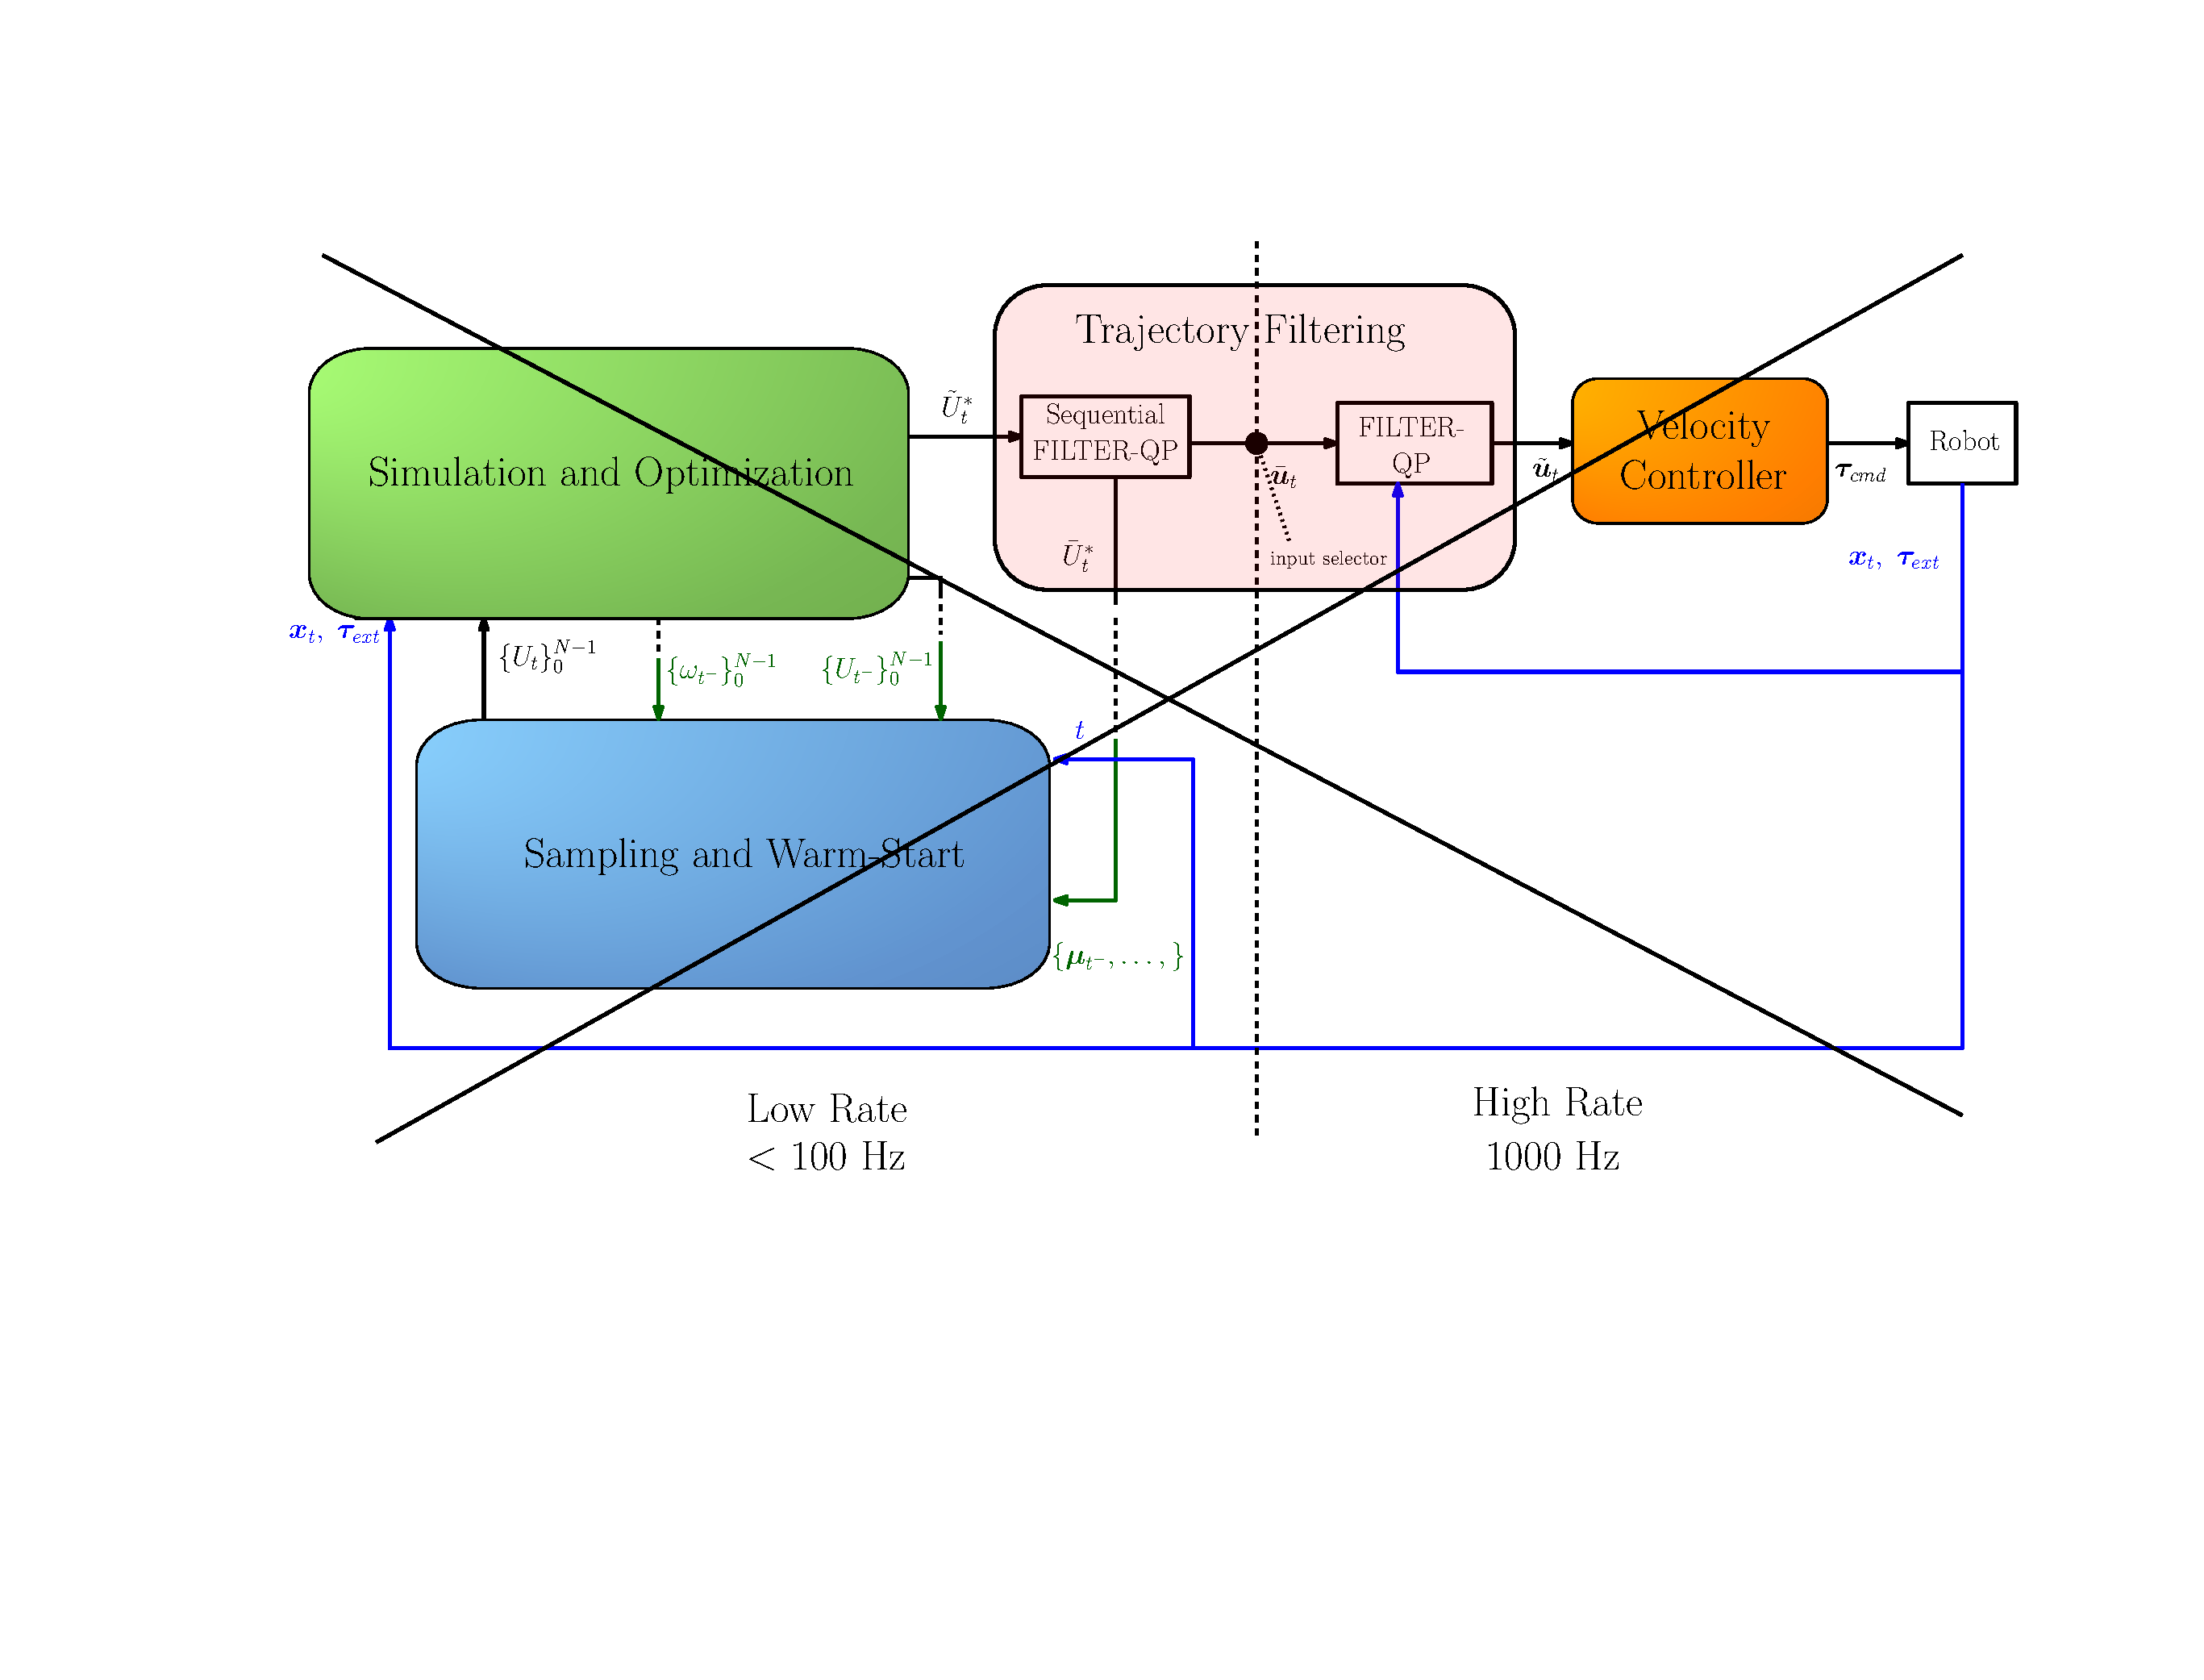
\includegraphics[width=0.95\columnwidth] {figures/schemes/receding_horizon_new_paper_sout.pdf}
% \hspace{1cm}
% \end{figure}
% \fi

\begin{figure}[t!]
\centering
\vspace{-0.5cm}
% \hspace*{-1.5cm}
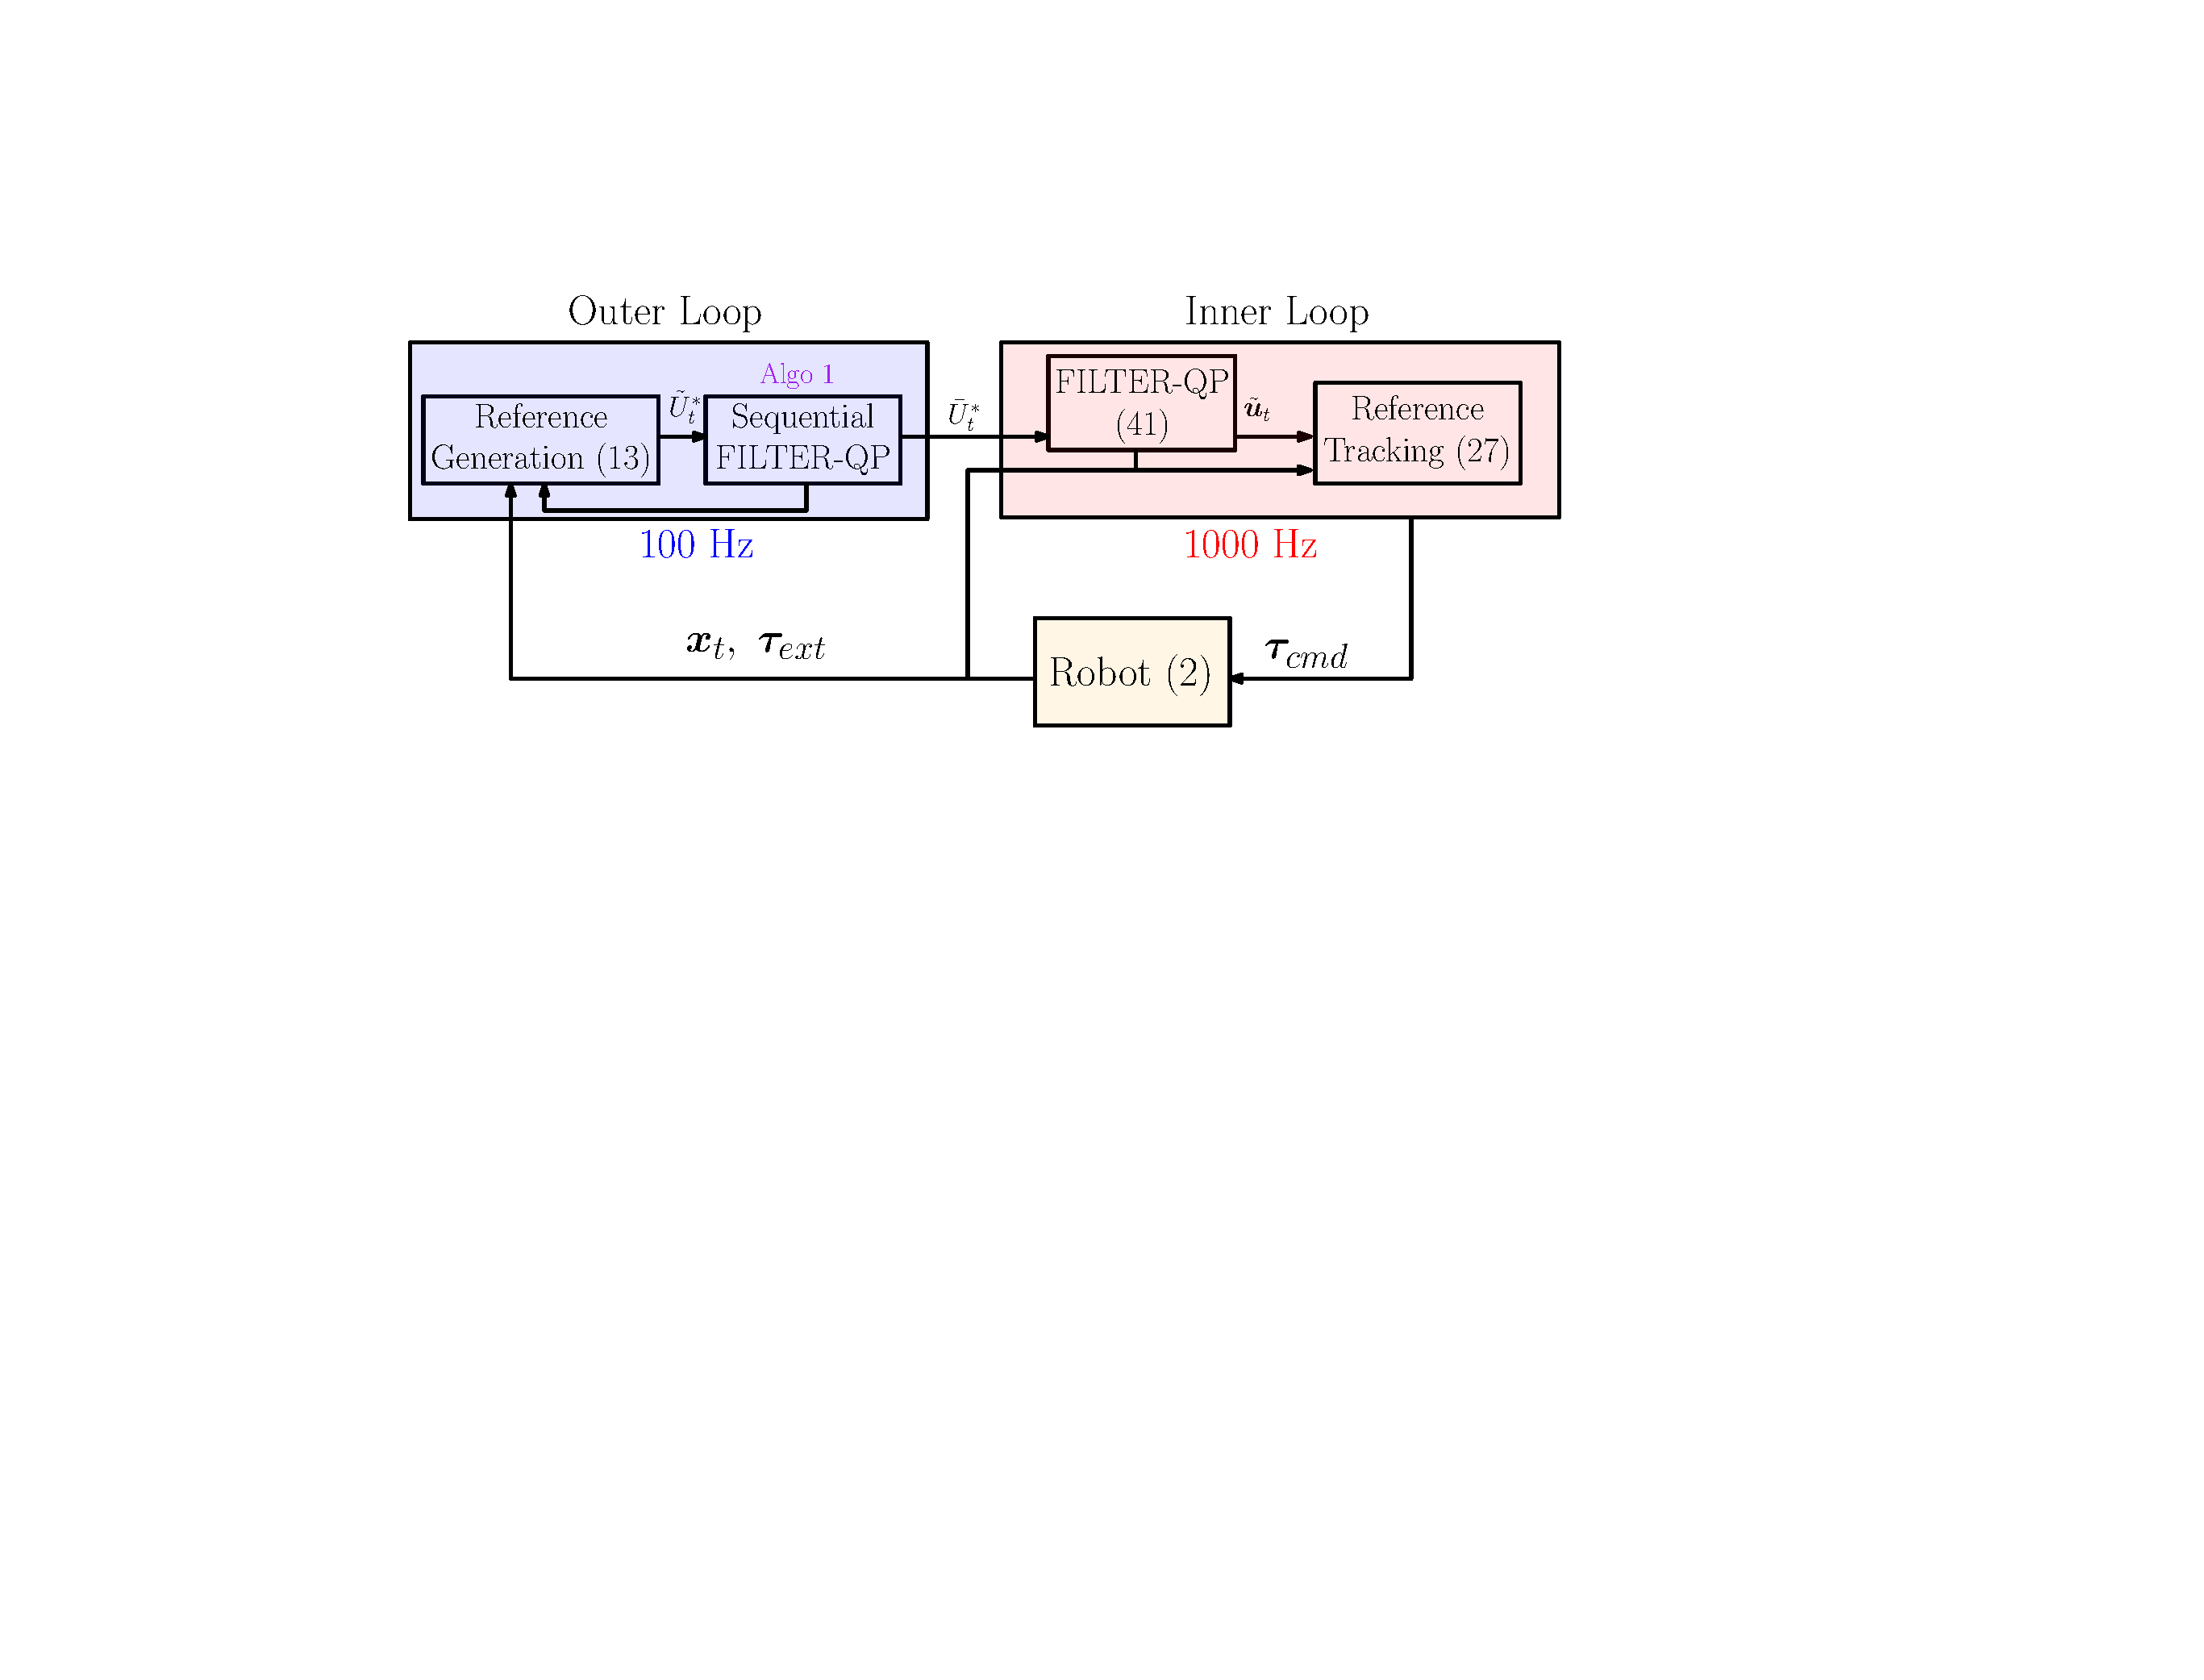
\includegraphics[width=0.95\columnwidth] {figures/schemes/receding_horizon_new_paper2.pdf}
\caption{The figure shows an high-level schematic of the method. \add{The outer loop generates safe trajectories at a low rate, while the inner loop tracks this reference enforcing that passivity and motion constraints are enforced at a higher rate. The outer loop block, including the details of the sampling procedure are further expanded in \fig\ref{fig:receding_horizon}.}} \label{fig:block_scheme}
\end{figure}


\add{In the following we present each component of the framework. We start by} presenting our cost formulation for the manipulation task. This is used in the reference generation sampling procedure to weight different trajectory samples and drive the robot to a successful task execution.

\add{Afterward}, we encode safety requirements in the form of ZBFs. \add{The} safety objectives \add{introduced} here are formulated on a kinematic level (obstacle avoidance, joint and Cartesian limits).

We are also interested in the robustness of the dynamical system during interaction, especially in cases of unexpected events that could compromise its stability. To this end, we complete the proposed framework with a passivity analysis and use an energy tank to bound the energy dissipated during the manipulation task. Passivity is guaranteed in the form of an additional constraint in the quadratic program and therefore naturally fits the proposed framework.

\add{We conclude with the description of the deployed low-level controller which tracks joint velocity references.}

\subsection{\add{Reference Generation}}
The sampling-based \add{controller samples reference commands for the low-level reference tracking controller. We decide to directly sample in the joint velocity space} to account for objectives which are not in the operational control space such as joint limits and self-collision avoidance. The internal model used to sample trajectory rollouts has the same form as in \eqref{eq:eom}.

As described in Section~\ref{sec:formulation}, the control objective is to drive the system to minimize a task-dependent cost function over time. Furthermore, as state constraints are not explicitly taken into account by the formulation, a common heuristic is to penalize deviations from feasible states in the cost function. In the following we define several cost components associated with the different high-level objectives and constraints.
We denote by $\mathds{1}[\vect{x}]$ the \textit{indicator function} such that,
\begin{equation}
    \mathds{1}[\vect{x}]_i = 
    \begin{cases}
    1 & \text{if } x_i \text{ is True} \\
    0 & \text{otherwise}.
    \end{cases}
\end{equation}
\add{with $\star_i$ the $i$\textsuperscript{th} element of vector $\vect{\star} \in \nR{n}$.}
In the following we drop from the notation the dependence on the current state. We use $\weightMatrix{}$ to denote positive semidefinite weight matrices and $\weightScalar{}$ for non-negative scalar parameters. Note that input constraints are not treated here as additional cost terms as the non-linear dynamics can be augmented with a function that projects the sampled inputs into the feasible set $\mathcal{U}$.

\paragraph{Target reaching} in the target reaching task, the goal is to bring a frame attached to the robot (generally the end-effector frame) to a desired pose. We define with $\matr{T} \in SE(3)$ and $\matr{T}^* \in SE(3)$ the current and desired target frame pose, respectively. The \textit{tracking cost} is computed as a weighted distance in the tangent space to $SE(3)$ using the logarithmic mapping~\cite{blanco2010tutorial}:
\begin{equation} \label{eq:tracking_cost}
     c_{t} = || \log(\matr{T} - \matr{T}^{*}) ||^2_{\weightMatrix{t}}.
 \end{equation}
 
 \paragraph{Collision avoidance} let $\contact \in \{0, 1\}$ represent an auxiliary variable which is equal to 1 when the manipulator is in contact with the environment. The value of $\contact$ can be computed searching for collisions between bodies. 
 \add{This cost term  is activated when we want to execute a contact-free motion of the end-effector}. 
 The \textit{contact cost} is defined as,
 \begin{equation}
     c_{\contact}= \weightScalar{\contact} \contact(\state).
 \end{equation}

 \paragraph{Joint position limits} the manipulator is subject to physical joint limits. These can be addressed by introducing a cost component that penalizes violation of the constraints. We define the \textit{joint limits cost} with:
 \begin{align}
     &c_{j} = \mathds{1}[\configRobot > \upperLimits]^T(\weightScalar{j} + ||\upperLimits - \configRobot||^2_{\weightMatrix{js}}) + \nonumber\\ 
     &\qquad\mathds{1}[\configRobot < \lowerLimits]^T(\weightScalar{j} +  || \configRobot - \lowerLimits||^2_{\weightMatrix{js}}), 
 \end{align}
 where the scalar $\weightScalar{j}$ is a constant cost added when the limit is violated. The matrix $\weightMatrix{js}$ adds a quadratic term in the limit violation. This was shown in~\cite{williams_information-theoretic_2018} to help the controller find its way back if poor sampling brings the system outside of the joint position limits.
 
 \paragraph{Arm reach} we introduce an additional term that penalizes configurations where the arm's end-effector moves excessively relative to the base 2D placement. This helps to bias solutions where base motion is preferred over stretching the arm which can lead to singular configurations. The translation vector from the end-effector frame $\mathcal{E}$ to the arm base frame $\mathcal{B}$ is defined with the vector $\vect{p}_{\mathcal{B}\mathcal{E}} \in \nR{3}$. The current reach is then $r_{\text{curr}} =  \vect{p}_{\mathcal{B}\mathcal{E}}^T \matr{P} \vect{p}_{\mathcal{B}\mathcal{E}}$. The projection matrix $\matr{P} = \text{diag}(1, 1, 0) \in \nR{3 \times 3}$ makes sure that the reach is only computed in the 2D plane. Given a maximum reach $r_{\text{max}} \in \nR{}_{\geq 0}$, the \textit{reach cost} is then defined by:
 \begin{equation}
   c_r = \mathds{1}[r_{\text{curr}} > r_{\text{max}}] (\weightScalar{r} + \weightScalar{rs}(r_{\text{curr}} - r_{\text{max}})^2).    
 \end{equation}

 \paragraph{Self-collision avoidance} similarly to arm reach, self-collision avoidance can be implemented as an additional cost term which is active when the distance between a pair of frames is less than a pair-dependent threshold. Given the distance between two frames $d_{ij}$ and a threshold $d^{min}_{ij}$ the self-collision cost for the pair is:
 \begin{equation}
   c_{sc} = \sum_{ij, i \neq j} \mathds{1}[d_{ij} < d^{min}_{ij}] (\weightScalar{r} + \weightScalar{rs}(d^{min}_{ij} - d_{ij})^2).    
 \end{equation}
 
 \paragraph{Object manipulation} in the manipulation task the goal is to change the state of an articulated object through interaction. The \textit{manipulation cost} penalizes deviations from the target object configuration $\configObject^{*}$,
\begin{equation}
    c_o(\configObject; \weightMatrix{o}) = || \configObject - \configObject^{*}||^2_{\weightMatrix{o}}.
\end{equation}
\paragraph{Power minimization} we propose a new cost component that takes into account the power dissipated to perform the task. In fact a successful interaction (i.e., opening the door) could happen in multiple ways, however trajectories that dissipate low power are most efficient as they do not act against the environment and robot kinematic constraints. We leverage the fact that as rollouts are performed in simulation, the joint torque generated through interaction can be easily computed by summing the contribution of each force $\vect{f}_c \in \nR{3}$ at each contact point $c$:
\begin{equation}
\boldsymbol{\tau}_{ext} = \sum\limits_{c} \matr{J}_c^T \vect{f}_c,    
\end{equation}
where $\matr{J}_c$ is the contact Jacobian. The power dissipated during the task is therefore $-\boldsymbol{\tau}_{ext}^T\command$, which is positive when acting ``against" the environment. The cost associated with power penalization is:
\begin{equation}
   c_p = \weightScalar{p} \cdot \max(0, - \boldsymbol{\tau}_{ext}^T\command - p_{max}),      
 \end{equation}
where $p_{max}$ is the maximum power that can be dissipated during the task.

\subsubsection{Cost Scheduling}
The manipulation task consists of two phases. In a first phase the manipulator reaches an estimated contact point, allowing for a fast and successful exploration in the following interaction phase. In the second phase, the goal is to bring the object to the desired state while keeping the end-effector close to the contact location. This switch is manually enabled by turning on the object manipulation cost $c_o$ after a successful approach. Reducing the end-effector position penalty during the manipulation phase allows the controller to choose a trajectory that fully exploits the contact dynamics by changing the hand pose.

%This approach is in contrast with previous works where manipulation generally follows a prescribed grasping state~\cite{abraham_model-based_2020}. Grasping introduces a kinematic constraint that, while reducing the optimal control search space, does not allow for more flexible, contact-based behaviors to emerge such as pulling, pushing or sliding. 

\subsection{\add{Safety Constraints}}
In the previous subsection a combination of cost components were introduced in order to address both performance and safety. The variety of objectives makes the cost landscape highly complex such that trading off performance against safety objectives can be quite challenging and tedious. Furthermore, as already stressed, sampling does not provide any formal guarantee that constraints encoded in the form of additional cost terms will be satisfied. Therefore, we look at how barrier functions can encode safety-critical constraints. As described in \cite{benzi2021optimization}, a simple ZBF can be derived for each joint to keep it between its lower and upper bounds, $q_i^-$ and $q_i^+$, respectively:
\begin{equation}
h_{ql}^i = \frac{(q_i^+ - q)(q - q_i^-)}{(q_i^+ - q_i^-)}\;.
\end{equation}

In the following we treat the safety requirements associated to robot frames and denote with $\vect{p}_{\mathcal{A}} \in \nR{3}$ the position of a generic robot frame $\mathcal{A}$ computed through forward kinematics. The ZBF constraint can then be derived using the differential kinematics equation,
\begin{equation}
    \dot{\vect{p}}_{\mathcal{A}} = \matr{J}^{lin}_{\mathcal{A}} \dconfigRobot\;,
\end{equation}
with $\matr{J}^{lin}_{\mathcal{A}}$ being the linear Jacobian associated with frame $\mathcal{A}$ and assuming that joint velocities are accurately tracked. 

The self-collision safe set can be obtained by approximating potentially colliding frames with non-intersecting spheres. Then the self-collision ZBF is defined as,
\begin{equation}
    h_{sc}^{ij} = \frac{1}{2}(||\vect{p}_{\mathcal{C}_i} - \vect{p}_{\mathcal{C}_j}||^2 - d_c^2),
\end{equation}
where $d_c = r_i + r_j$ is the sum of the radius of the two collision spheres associated with the $i$\textsuperscript{th}  and $j$\textsuperscript{th} collision pair frames. Note that we can similarly encode arm reach limits. In fact, the following is a valid ZBF, positive only when the end-effector is within the prescribed maximum reach $r_{max}$ with respect to the arm base,
\begin{equation}
    h_{ar} = \frac{1}{2}(r_{max}^2 - (\vect{p}_{\mathcal{E}} - \vect{p}_{\mathcal{B}})^T \vect{P} (\vect{p}_{\mathcal{E}} - \vect{p}_{\mathcal{B}}) ).
\end{equation}
The projection matrix $\vect{P} = \text{diag}(1, 1, 0) \in \nR{3 \times 3}$ makes sure that the reach is only computed in the 2D plane. This prevents the arm from stretching out and reaching singular configurations. Each of these ZBFs translates to a constraint of the form in \eqref{eq:cbf-const} which is affine in the commands. 

As described in \sect \ref{sec:theory}, we can formulate a quadratic program to find the command which is the closest to the sampled one while also satisfying the ZBF constraints previously introduced:
\begin{mini}|s| 
{\tilde{\vect{u}}_t, \boldsymbol{\delta}}{||\tilde{\vect{u}}_t - \command_t||^2 + \boldsymbol{\delta}^T \matr{\Gamma} \boldsymbol{\delta}\quad \text{(FILTER-QP)}}{}{\label{eq:cbf-qp}}
\addConstraint{\dot{h}^i_{ql} \geq -\gamma{h}_{ql} + \delta^i_{ql} \quad \forall \ i \in [1,  m] }{}{\ \text{(Joint Limits)}}
\addConstraint{\dot{h}^{ij}_{sc} \geq -\gamma{h}_{ij} + \delta^{ij}_{sc} \quad \forall \ (i,j) \in \mathcal{I}}{}{\ \text{(Self Collision)}}
\addConstraint{\dot{h}^i_{ar} \geq -\gamma{h}_{ar} + \delta^i_{ar}}{}{\ \text{(Arm Reach)}}
\addConstraint{\tilde{\vect{u}}_t \in \mathcal{U}}{}{ \text{\ (Input Limits)}},
\end{mini}
where $\boldsymbol{\delta}$ is the vector of slack variables and $\matr{\Gamma}$ is a positive definite diagonal matrix weighting the slack variable penalization whose dimensions depend on the number of implemented soft constraints. 
\add{
\begin{rmk} 
Note that slack variables might cause a violation of the constraint. We address this problem using more conservative limits, allowing for a small constraints violation at the constraint boundary. In particular if $\tilde{h}$ is the original ZBF, we deploy a stricter barrier funztion $h = \tilde{h} - \Delta$ with $\Delta \geq 0$. Imposing that the slack variables are bounded from below:
\begin{equation} \label{eq:slack_bound}
    \delta > -\gamma \Delta,
\end{equation}
the ZBF constraints can be rewritten as:
\begin{equation}
    \dot{\tilde{h}} = \dot{h} \geq  -\gamma h + \delta = -\gamma \tilde{h} +\gamma \Delta + \delta \geq  -\gamma \tilde{h}. 
\end{equation}
Therefore satisfying the constraint on a stricter set \emph{with} bounded slack variables, implies satisfying the hard ZBF constraint on the original larger invariant set:
\begin{equation}
\dot{h} \geq -\gamma h + \delta \quad\Rightarrow \quad\dot{\tilde{h}} \geq -\gamma \tilde{h}.    
\end{equation}
One can tune the stricter safe set such that the slack variable does not get smaller than the safety margin $-\gamma\Delta$. Practically, for our conservative choice of safe set, the constraints on the slack variables are always satisfied, thus we can solve the simpler optimization in \eqref{eq:cbf-qp}.
\end{rmk}
} Finally, the set denoted by $\mathcal{I}$ is the set of collision link pairs.  We name this problem FILTER-QP as it changes the control input only if it is unsafe. Instead of simply applying this optimization point-wise, we can \emph{filter} the full input sequence in a sequential manner. After a policy update and for each time step, a FILTER-QP is solved. The newly computed command is applied to advance to the next step in the horizon and obtain the next system state from which the constraint equation can be updated. We call this procedure Sequential FILTER-QP and describe it in \algo \ref{algo:sequential_qp}. The resulting filtered optimal input sequence $\bar{U}^*_t$ is then also used to warm-start the nominal policy for the next round of rollout sampling (see \fig \ref{fig:receding_horizon}). The reader can also refer to \fig~\ref{fig:block_scheme} for a schematic representation of the complete feedback control loop.

\begin{algorithm}
\caption{Sequential FILTER-QP \label{algo:sequential_qp}}
\KwData{optimal input sequence $U^*_t = \{ \command^*_t, \dots, \command^*_{t+T-\Delta t}\} = \{\boldsymbol{\mu}_t, \dots, \boldsymbol{\mu}_{t+T-\Delta t}\}$ , current state $\vect{x}_t$, simulation steps $K$
%tank state $x_t$
}
\KwResult{filtered input trajectory $\bar{U}^*_t$}
$\vect{x} \gets \vect{x}_t$\;
$\command \gets \command^*_t$\;
$k \gets 0$\;
\While{$k < K$}{
  $\bar{\command}_{t+k\Delta t} \gets \text{FILTER-QP}(\vect{x}, \command, \boldsymbol{\tau}_{ext})$ \hfill (\eqn \ref{eq:cbf-qp}) \\
  $\vect{x}, \boldsymbol{\tau}_{ext} \gets $Step Simulation \hfill (\eqn \ref{eq:eom})\\
  %$x_t \gets$ Integrate Tank \hfill (\eqn \ref{eq:tank_dynamics}) \\
  $k = k + 1$ \\
  $\command \gets {\command}^*_{t + k\Delta t}$
}
\end{algorithm}

\subsection{\add{System Stability}}
While the optimization in \eqref{eq:cbf-qp} enhances the safety of the system we still lack stability guarantees. As described in \sect \ref{sec:theory}, energy tanks can be used to make the system \emph{passive} and thus ensure stability. Inspired by the work in \cite{benzi2021optimization} and \cite{shahriari2018valve}, this adaptation naturally fits the control method we have developed so far. If we augment the optimization problem in \eqref{eq:cbf-qp} with the energy constraint:
\begin{equation}\label{eq:pass_const}
    \int\limits_{0}^{t} \boldsymbol{\tau}_{ext}^T \dconfigRobotDesired \ d\tau \geq -S_{tank}(0),
\end{equation}
where $S(0)$ is the initial energy stored in the tank, then the following stability result holds:

\begin{theorem}[Controlled System Stability]
If the optimization problem FILTER-QP satisfies constraint \eqref{eq:pass_const}, then the controller makes the system \eqref{eq:eom} passive and therefore stable. 
\end{theorem}

\begin{proof}
We start by augmenting the system model with a virtual tank. We now need to define through which \emph{power ports} the tank exchanges energy with the rest of the system. To this end, we perform a passivity analysis of the \emph{real} system. We first define the robot energy as, 
\begin{equation}
    S_{robot} = \frac{1}{2} \dconfigRobotError^T \massMatrix \dconfigRobotError + \frac{1}{2} \configRobotError^T \matr{K}_I \configRobotError.
\end{equation}
In order to study the passivity of the system, we need to derive the robot energy dynamics $\dot{S}_{robot}$. A complete derivation can be found in the Appendix~\ref{app:passivity_analysis}. It turns out that:
\begin{equation}
    \dot{S}_{robot} = \dconfigRobotError^T \externalTorque - \dconfigRobotError^T \matr{K}_D \dconfigRobotError \leq \dconfigRobotError^T \externalTorque. 
\end{equation}
The power flow through the external torque has indefinite sign and can lead to a loss of passivity. Since the environment is passive, there exists an environment energy $\dot{S}_{env}$ such that~\cite{shahriari2018valve},
\begin{equation}
    \dot{S}_{env} \leq -\dconfigRobot^T \externalTorque.
\end{equation}
The energy tank is finally connected to the system through the power port $(\dconfigRobot^*, \externalTorque)$ and therefore,
\begin{equation} \label{eq:tank_dynamics}
\dot{S}_{tank} = \dconfigRobot^{*T} \externalTorque. 
\end{equation}
Then, the energy evolution of the autonomous system, composed of robot, tank and environment is,
\begin{equation} 
\begin{aligned} \label{eq:autonomous_sys_energy}
    \dot{S}_{tot} &= \dot{S}_{robot} + \dot{S}_{tank} + \dot{S}_{env} \\
    &\leq \dconfigRobotError^T \externalTorque + \dconfigRobot^{*T} \externalTorque - \dconfigRobot^T \externalTorque \leq 0,
\end{aligned}
\end{equation}
showing the system's passivity.
Intuitively, the increase of the robot's energy is compensated with a reduction of the tank's energy. 
\add{Therefore the total energy stored in the system is bound by $S_{tank}(0) + \Lambda$ with $
\Lambda$ some positive constant.} \add{In order for \eqref{eq:autonomous_sys_energy} to be valid we are relying on the silent assumption that the robot is able to exchange energy with the tank at any time. As the tank energy is a positive definite quantity and therefore bounded from below, we need to ensure that it is never completely depleted, imposing:}
\begin{equation} \label{eq:pass_cond}
    S(t) = S(0) + \int_{0}^{t} \boldsymbol{\tau}_{ext}^T \dconfigRobotDesired \ d\tau  \geq 0,
\end{equation}
recovering the constraint in \eqref{eq:pass_const} therefore concluding the proof. \add{In other words, \eqref{eq:pass_cond} is a condition that is required for \eqref{eq:autonomous_sys_energy} to hold at any time.}
\end{proof}
In practice, the constraint in \eqref{eq:pass_const} is formulated as
\begin{equation}
    \int_{0}^{t} \boldsymbol{\tau}_{ext}^T \command \ d\tau \geq \epsilon - S(0),
\end{equation}
where $\epsilon$ is a positive minimum residual energy to avoid the singularity that the tank suffers when it is completely depleted.  

\subsection{\add{Low-level Controller}}
\add{Finally we describe the low-level control law. We consider a dynamic manipulator as described in \eqref{eq:eom}. The robot uses a dynamically compensated low-level velocity controller to convert a velocity reference in torque commands:}
\begin{equation} \label{eq:low-level-control}
\commandTorque = \add{\massMatrix \ddconfigRobotDesired} + \coriolis \dconfigRobotDesired + \vect{g}_r(\configRobot) - \matr{K}_D \dconfigRobotError - \matr{K}_I \int_{0}^{t} \dconfigRobotError\ d\tau,
\end{equation}
\add{with the auxiliary error variable $\configRobotError =  \configRobot - \configRobotDesired$ and $\matr{K}_D$ and $\matr{K}_I$ being positive diagonal gain matrices.}